%=====================================================================
\section{Active circles: the $+1$ bulk and the wall layer}\label{sec:ccharge}
\subsection{Fixed size, all windings: $R=1.43\,\la$, $k=2\dots10$}
The cleanest test: $R=31.83$ ($R/\la=1.43$), $k=2\dots10$ ($\rho=0.02$--0.10, $\rho\la=0.44$--2.2), 3 seeds, 10k warm-up + 40k
steps. Two independent edge rules (Sec.~\ref{sec:edge}): the density minimum $d_\rho$ and the pinned-site rule.
\begin{table}[H]\centering\small
\caption{Fixed-radius scan, mean $\pm$ s.e.\ over 3 seeds. $q_b$: bulk charge per frame; $P_1$: fraction of frames with
$q_b=+1$ exactly; $d_\rho$: density-minimum edge (cells from the wall); $N_L$: $+\half$ in the layer; sites: pinned sites
found; agree: fraction of $+\half$ classified identically by the two rules. Last two columns: the passive layer width
used as the edge instead, which fails (Sec.~\ref{sec:passive}).}\label{tab:rscan}
\begin{adjustbox}{max width=\textwidth}
\begin{tabular}{rcccccccc|cc}\toprule
$k$ & $q_b$ (density) & $P_1$ & $d_\rho$ & $N_L$ & sites & $q_b$ (sites) & $P_1$ (sites) & agree & $q_b$ (passive edge) & $P_1$\\\midrule
2 & $1.03\pm0.02$ & 0.83 & 4.6 & 1.9 & 2 & $1.01\pm0.01$ & 0.91 & 0.956 & $0.44\pm0.05$ & 0.26\\
3 & $1.01\pm0.01$ & 0.90 & 4.2 & 4.0 & 4 & $1.03\pm0.01$ & 0.89 & 0.981 & $0.83\pm0.01$ & 0.69\\
4 & $0.99\pm0.00$ & 0.92 & 4.2 & 6.0 & 6 & $1.01\pm0.00$ & 0.94 & 0.990 & $0.98\pm0.01$ & 0.92\\
5 & $0.99\pm0.01$ & 0.90 & 4.2 & 8.0 & 8 & $1.02\pm0.01$ & 0.93 & 0.992 & $1.04\pm0.02$ & 0.90\\
6 & $1.01\pm0.01$ & 0.90 & 4.1 & 10.0 & 10 & $1.02\pm0.01$ & 0.94 & 0.993 & $1.07\pm0.01$ & 0.85\\
7 & $1.01\pm0.02$ & 0.89 & 4.2 & 12.0 & 12 & $1.05\pm0.02$ & 0.91 & 0.994 & $1.15\pm0.03$ & 0.74\\
8 & $1.00\pm0.00$ & 0.95 & 3.8 & 14.0 & 14 & $1.01\pm0.00$ & 0.96 & 0.997 & $1.18\pm0.01$ & 0.68\\
9 & $1.01\pm0.01$ & 0.94 & 3.8 & 16.0 & 16 & $1.02\pm0.02$ & 0.95 & 0.997 & $1.17\pm0.03$ & 0.71\\
10 & $1.04\pm0.03$ & 0.89 & 3.8 & 17.9 & 18 & $1.09\pm0.06$ & 0.90 & 0.994 & $1.20\pm0.04$ & 0.71\\\bottomrule
\end{tabular}
\end{adjustbox}
\end{table}
\begin{itemize}
  \item \textbf{The bulk carries $+1$ at every $k$}, to within 0.04, and is exactly $+1$ in 83--96\% of frames. The layer holds
        $N_L=2k-2$ of the $+\half$ (charge $k-1$) on exactly $2k-2$ pinned sites. The two rules agree on 96--99.7\% of all
        $+\half$; the lowest agreement is at $k=2$, where the layer is diffuse.
  \item The fluctuations are dynamical $\pm\half$ pairs (1.5--2.0 per frame) and occasional transients (one seed at $k=10$).
        Every run has a strong steady vortex (circulation order parameter $\Phi=0.89$--0.97).
  \item \textbf{The effect does not fade at low density} (H2 not supported): $q_b=+1$ down to $\rho=0.02$ ($\rho\la=0.44$),
        far below the predicted crossover $\rho\la\approx1$.
  \item A fixed cut 2.5 cells from the wall splits the layer and reports 1.2--1.5; the passive layer width is the wrong edge
        too (last columns). The bulk/layer boundary has to come from the active data themselves.
\end{itemize}
\begin{figure}[H]\centering
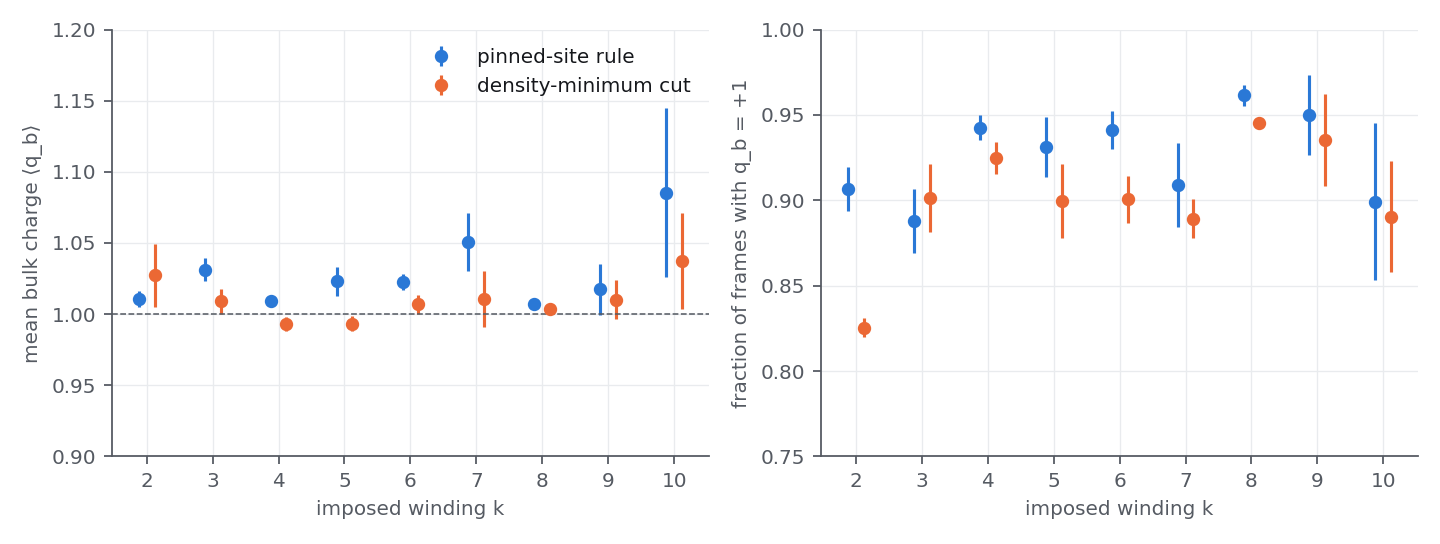
\includegraphics[width=0.85\textwidth]{circle_bulkcharge_rules.png}
\caption{Fixed-radius scan ($R=1.43\,\la$, 3 seeds): mean bulk charge (left) and fraction of frames with $q_b=+1$ (right) against $k$, pinned-site rule (blue) and density-minimum cut (orange).}\label{fig:rules}
\end{figure}

\subsection{Cut-free criteria: mobility and tilt}
Wall defects are slow and tilted; bulk defects are fast and point elsewhere (methods: Sec.~\ref{sec:edge}).
\begin{figure}[H]\centering
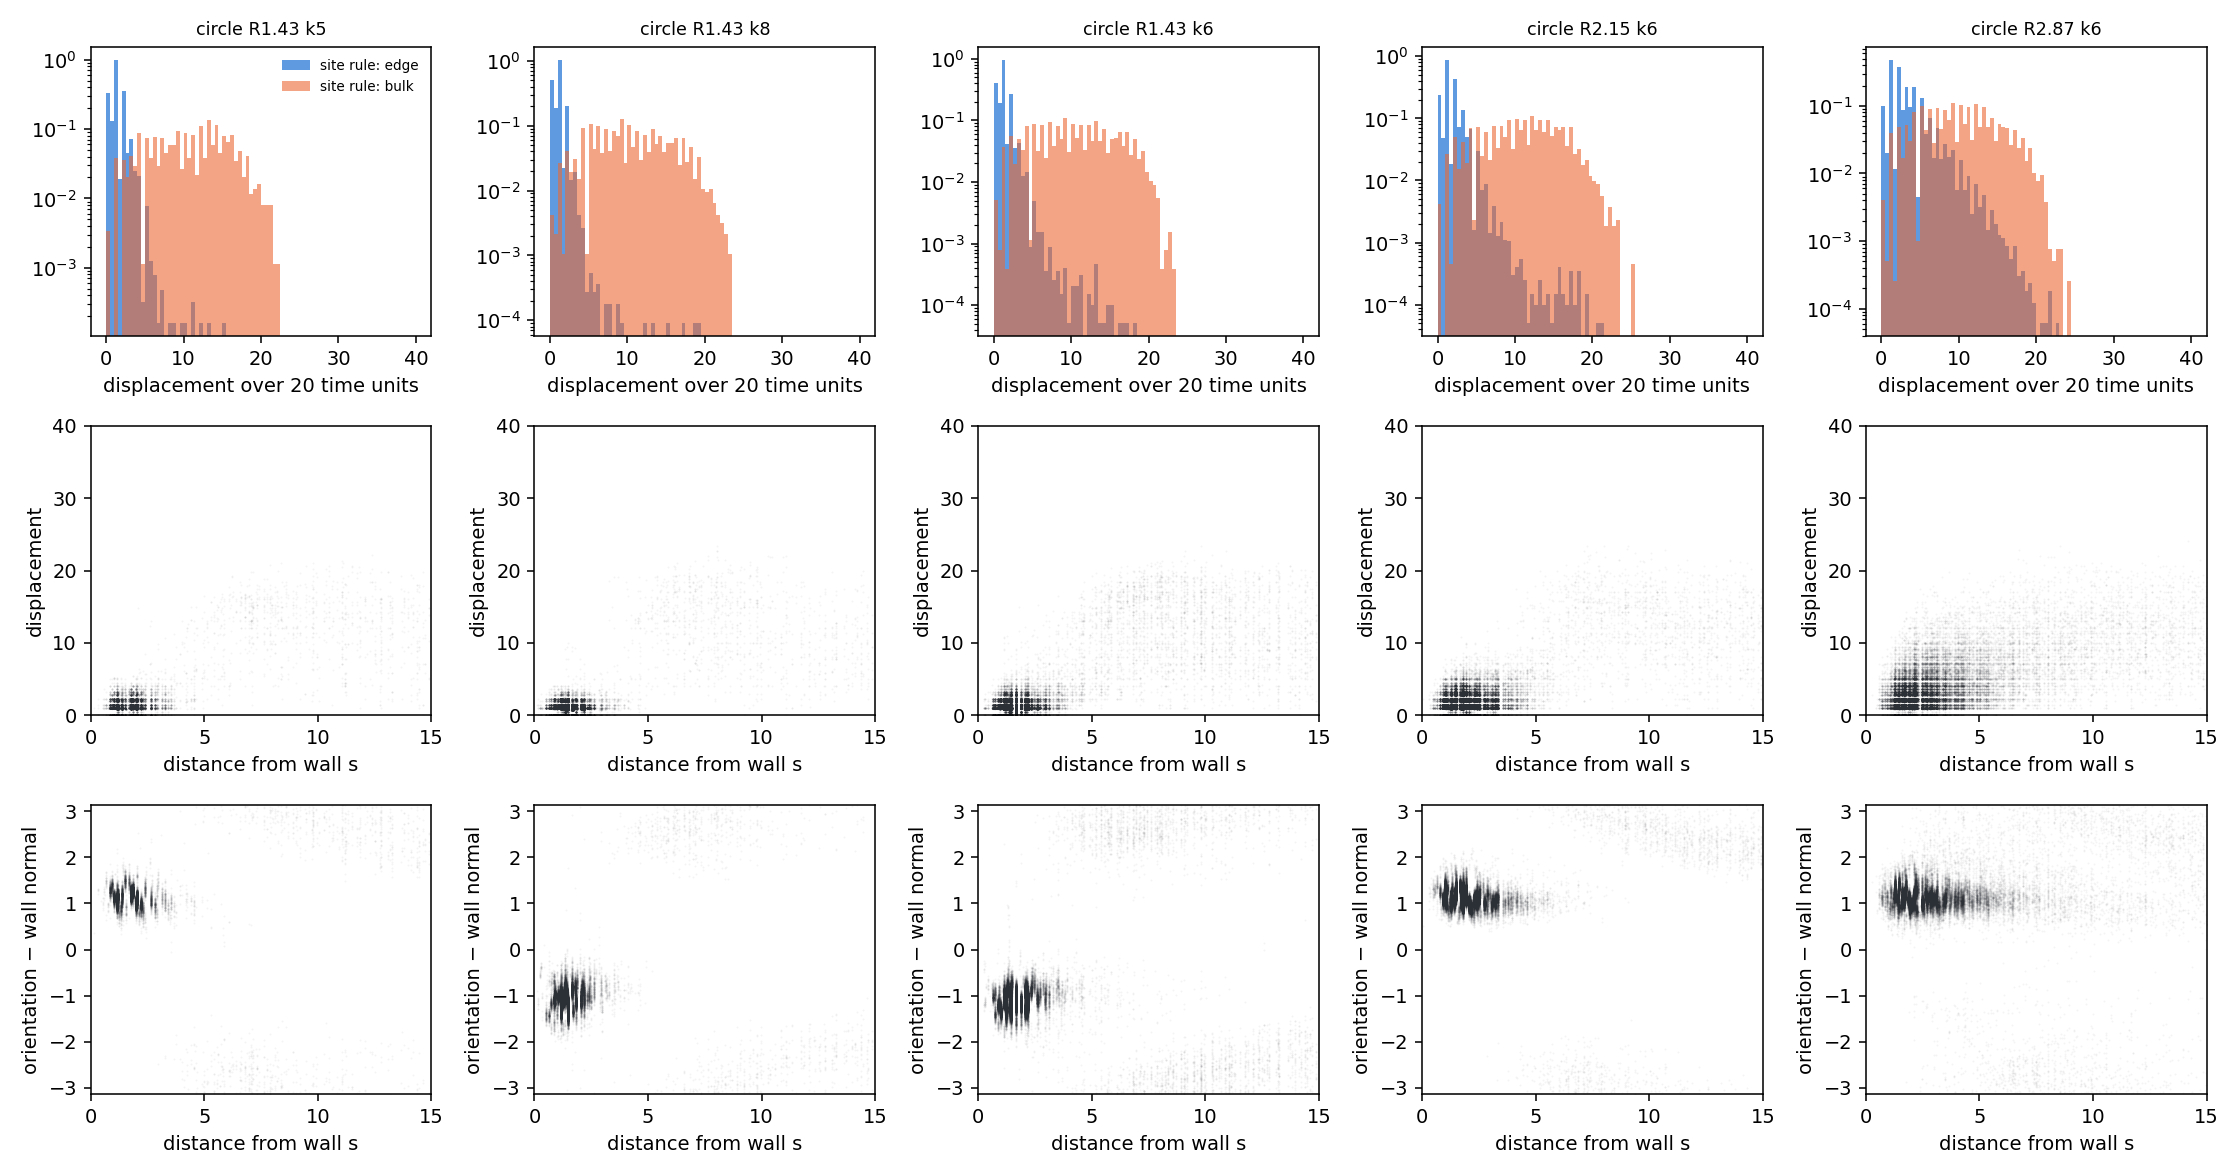
\includegraphics[width=\textwidth]{edge_criteria_circles.png}
\caption{Cut-free criteria on circles ($k=6$). Top: displacement over 20 time units, split by the site rule. Middle and
bottom: displacement and orientation relative to the outward wall normal against the distance from the wall.}\label{fig:crit}
\end{figure}
\begin{itemize}
  \item Wall defects: median displacement over 20 time units 1.0--1.4 cells against 10--11 in the bulk.
  \item \textbf{Tilt:} wall $+\half$ point at $|\Delta|\approx1.1$ rad ($\approx63^\circ$) from the outward normal, with the sign of
        the vortex sense in 6/6 runs; bulk $+\half$ cluster near $|\Delta|\approx\pi-0.5$. Nearly independent of $k$.
  \item Each criterion alone agrees with the site rule on 97--99\% of $+\half$ up to $2.15\,\la$ (89\% at $2.87\,\la$). With
        mobility, tilt or both, $q_b$ ($k=6$) is 1.05--1.07 at $1.43\,\la$, 1.11--1.25 at $2.15\,\la$ and 1.9--2.7 at $2.87\,\la$
        (site rule 1.85; part of the layer is tilted but mobile there).
\end{itemize}

\subsection{The whole parameter plane: main sweep}\label{sec:sweep}
834 active runs ($k=1$--20, $\rho=0.03$--0.50, 3 seeds; 10k + 100k steps) and 278 passive references. Every run was analysed
with the knee of $Q(r)$ (Sec.~\ref{sec:methods-knee}), $d^*$, $f^*$, the site rule and the wall Fourier analysis.
\begin{figure}[H]\centering
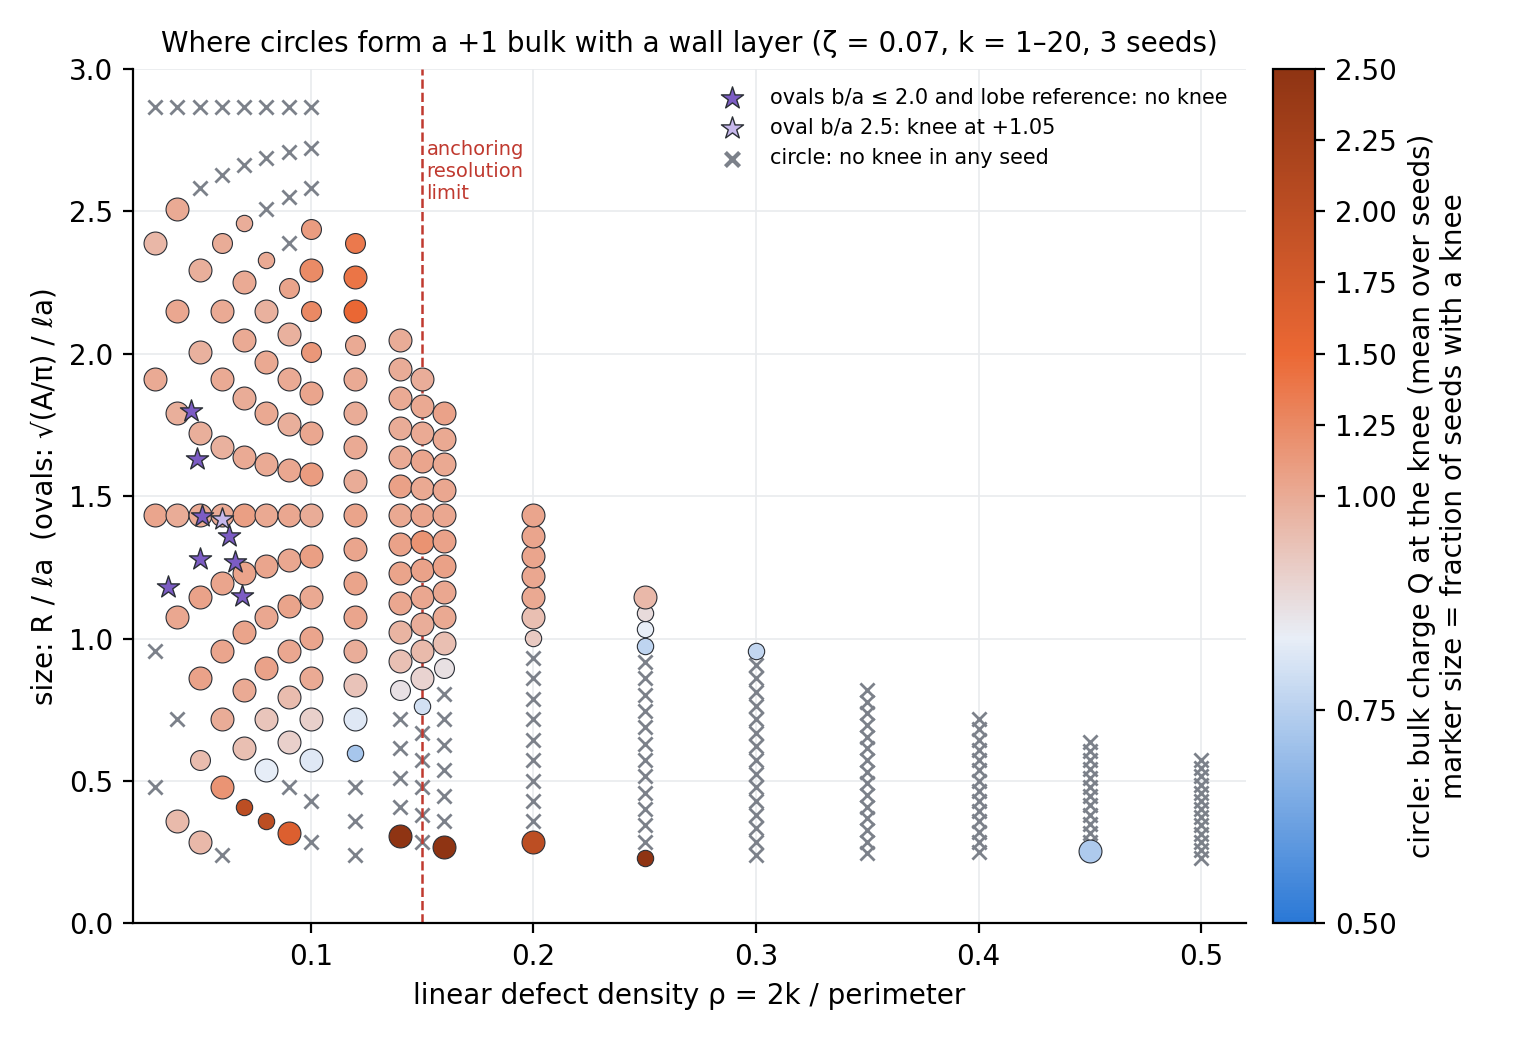
\includegraphics[width=0.85\textwidth]{layer_diagram_circles.png}
\caption{\textbf{Where circles have a $+1$ bulk and a wall layer.} Bulk charge at the knee of $Q(r)$ (colour; marker size =
fraction of seeds with a knee; crosses: no knee) over the linear defect density $\rho$ and the size $R/\la$. Stars: the
ovals at their own $\rho$ and equivalent radius $\sqrt{A/\pi}/\la$ (Part III).}\label{fig:diagram}
\end{figure}
\begin{table}[H]\centering\small
\caption{Main sweep, $\rho\le0.15$, all $k$, by size: fraction of runs with a knee, mean $Q$ at the knee, mean static
fraction of the wall lattice (1 = pinned; Sec.~\ref{sec:clattice}) and mean layer depth.}\label{tab:sweep}
\begin{adjustbox}{max width=\textwidth}
\begin{tabular}{lccccc}\toprule
$R/\la$ & runs & knee & $Q_\mathrm{knee}$ & $f_\mathrm{static}$ & $d^*/\la$\\\midrule
0.00--0.50 & 57 & 0.70 & 1.86 & 0.39 & 0.08\\
0.50--0.75 & 48 & 0.60 & 1.00 & 0.69 & 0.11\\
0.75--1.00 & 45 & 0.89 & 1.11 & 0.78 & 0.14\\
1.00--1.25 & 51 & 1.00 & 1.04 & 0.84 & 0.18\\
1.25--1.50 & 51 & 1.00 & 1.05 & 0.93 & 0.19\\
1.50--2.00 & 90 & 1.00 & 1.02 & 0.97 & 0.19\\
2.00--2.50 & 69 & 0.90 & 1.16 & 0.93 & 0.28\\
2.50--3.00 & 54 & 0.15 & 1.17 & 0.79 & 0.55\\\bottomrule
\end{tabular}
\end{adjustbox}
\end{table}
\begin{itemize}
  \item \textbf{Layer region: $R\approx0.75$ to $2$--$2.3\,\la$, at every density up to the resolution limit} (knee in 89--100\%
        of runs, $Q_\mathrm{knee}\approx1.0$, $f_\mathrm{static}\ge0.78$, $d^*\approx0.2\,\la\approx4.5$--6 cells).
  \item \textbf{Large cavities} ($\gtrsim2.5\,\la$): knee in 15\% of runs; the layer thickens ($d^*/\la=0.55$) and loses part
        of its sites. Degradation starts earlier at high $\rho$ (2.0--2.5\,$\la$: 42--48\% knees at $\rho\approx0.09$--0.13,
        100\% at low $\rho$).
  \item \textbf{Small cavities} ($\lesssim0.5$--$0.6\,\la$): no room for a bulk. The knee value tends to $k$ or is absent
        (e.g.\ $k=2$ at 0.36--0.48\,$\la$: knee at 1.6--2.0, i.e.\ no bulk pair at all).
  \item \textbf{Smallest clean circles} (the inscribed-radius test for the ovals, $\rho\approx0.06$): $k=3$, $R=0.72\,\la$:
        $Q_\mathrm{knee}=1.03$, $f_\mathrm{static}=0.97$, $d^*=0.16\,\la$; $k=4$, $0.96\,\la$: 1.07, 0.98, 0.17.
  \item Beyond the resolution limit ($\rho\ge0.2$) mostly no knee.
  \item \textbf{Knee finder:} with 5 smoothing bins it caught the flat shoulders of the cell-quantised layer steps (e.g.\
        $k=5$ at 0.80--0.90\,$\la$ gave a spurious knee at $Q\approx1.9$); 9 bins (0.045 in $r/R$) fixes it without moving genuine knees (Fig.~\ref{fig:knee}).
\end{itemize}
\begin{figure}[H]\centering
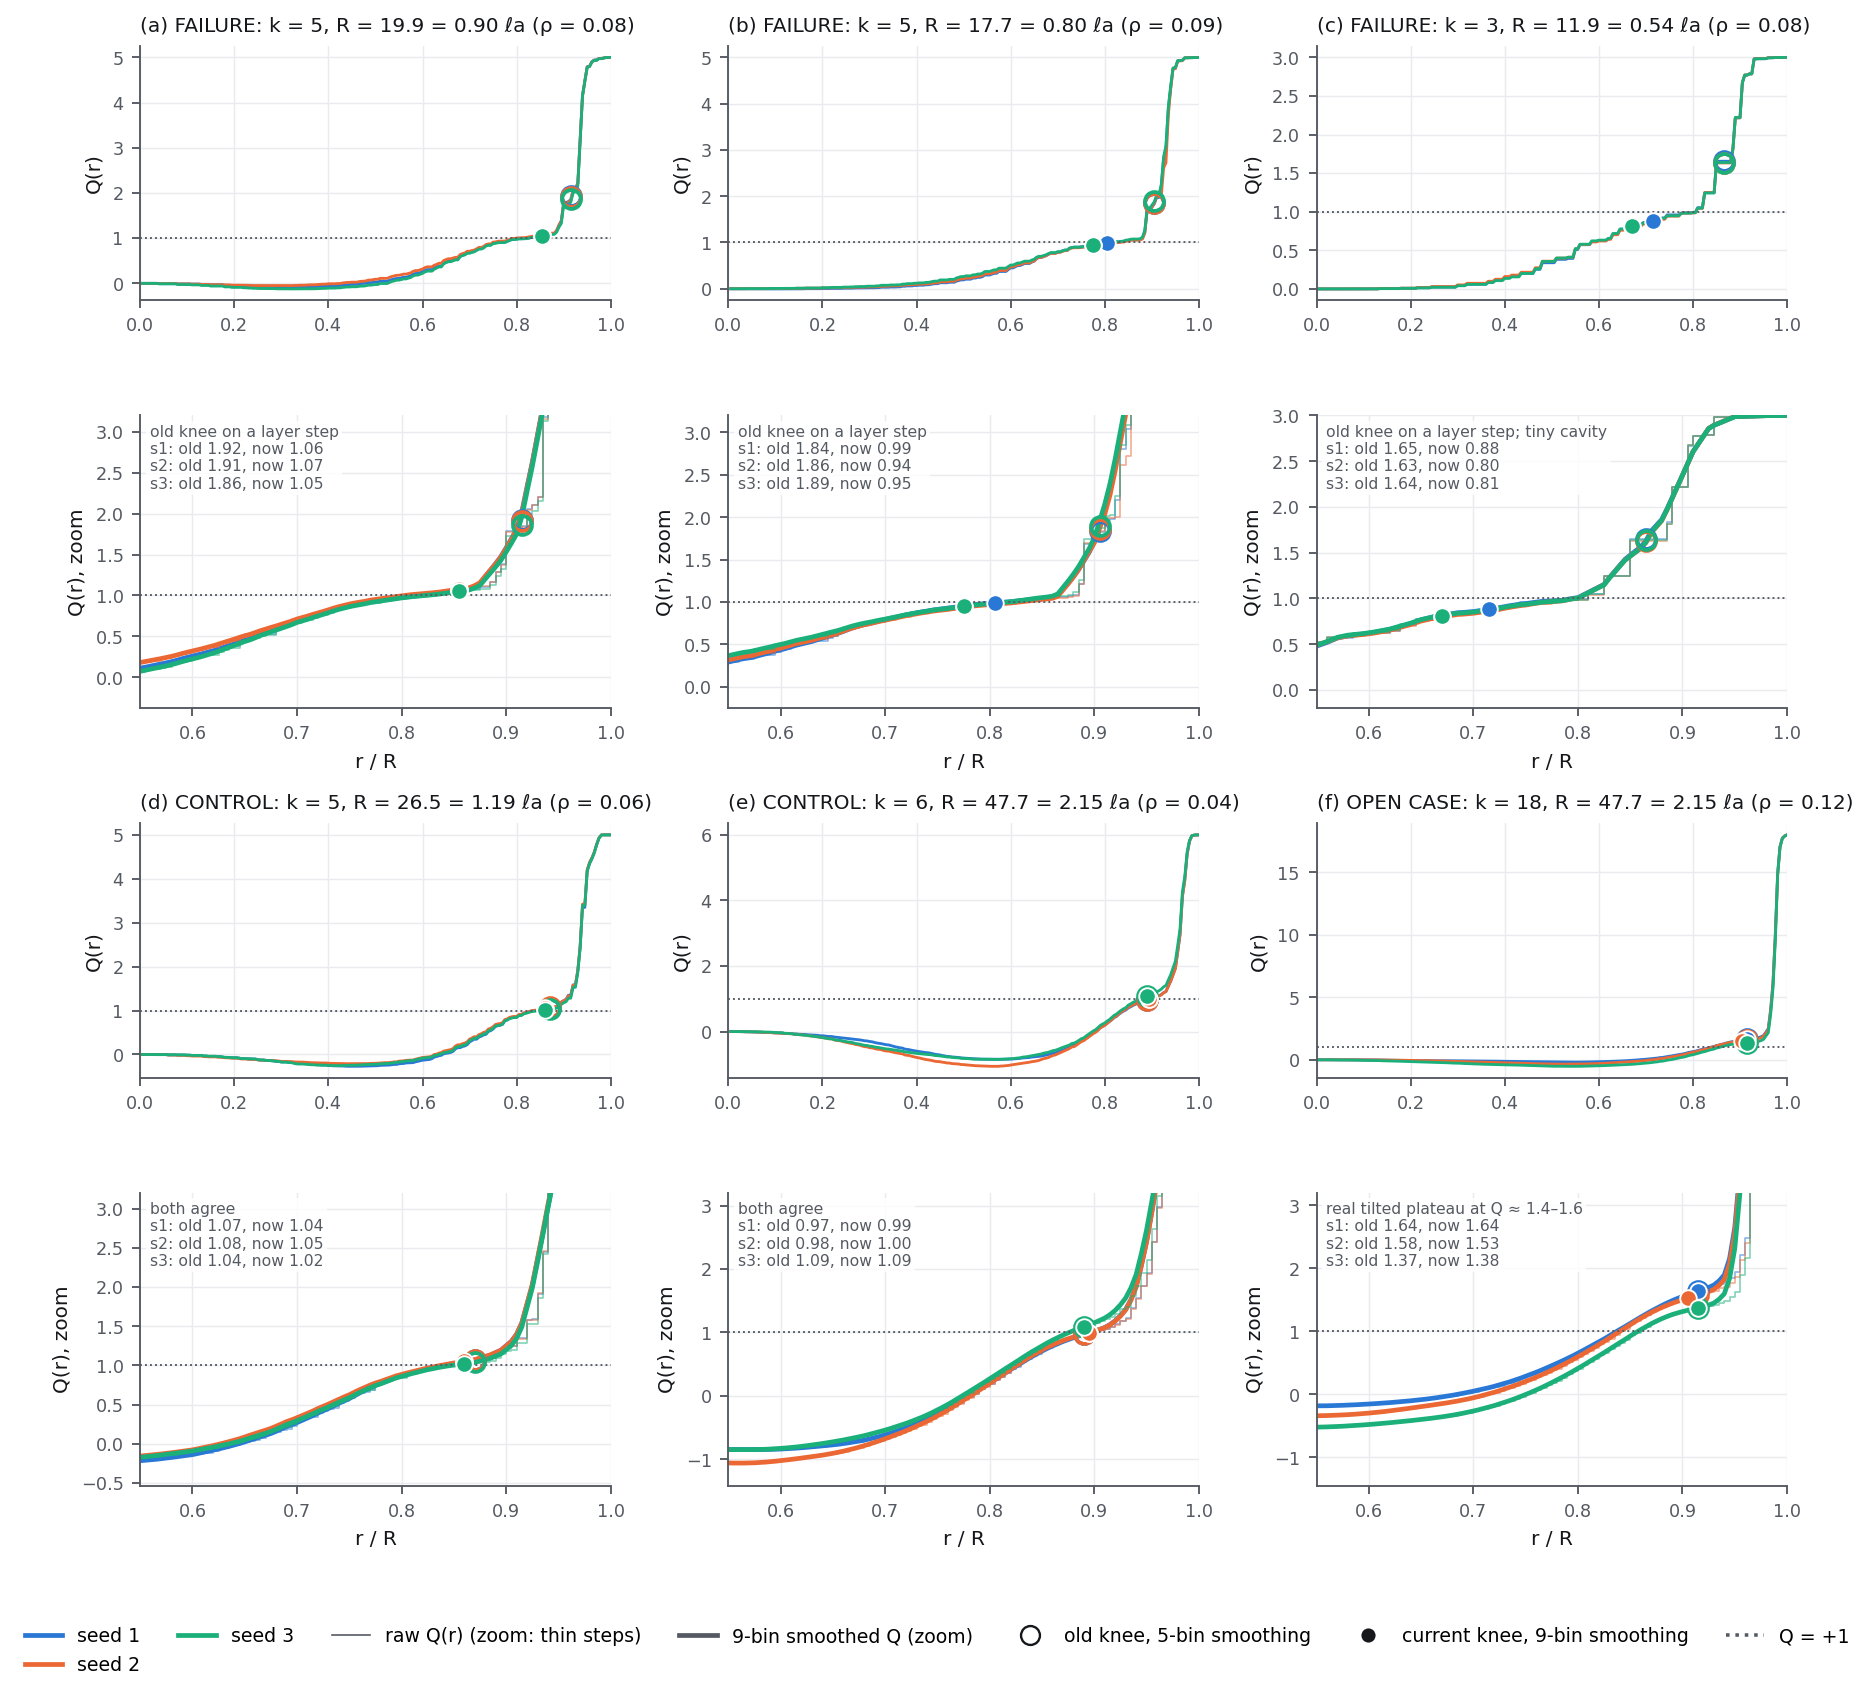
\includegraphics[width=\textwidth]{knee_check_v2.png}
\caption{\textbf{Why the knee finder smooths over 9 bins.} Six circles from the main sweep, three seeds each (blue, orange, green;
the seeds mostly overlap). For each run the upper panel shows the whole accumulated charge $Q(r)$ and the lower panel zooms on the
outer region, with the raw $Q(r)$ (thin steps) and the 9-bin smoothed $Q$ (thick). Open circles: knee found with the old 5-bin
smoothing; filled circles: knee with the current 9-bin smoothing (0.045 in $r/R$). The values per seed are printed in each zoom.
Close to the wall $Q$ climbs from $+1$ to $k$ in small steps, one per wall defect, each about 0.02 wide in $r/R$ because positions
are known to one cell.
(a, b) \emph{Failures of the old setting} ($k=5$, $R=0.90$ and $0.80\,\la$): with 5 bins a flat step part-way up the jump passes as a
plateau, and the finder reports a bulk charge of 1.84--1.92; 9 bins average the steps away and the knee moves inwards to the real
plateau, $Q=0.94$--1.07.
(c) \emph{Failure, and a limit of the method} ($k=3$, $R=0.54\,\la$): the old knee sits on a step at $Q\approx1.64$; the current knee
(0.80--0.88, at $r/R\approx0.7$) is better but still not the flattest part of $Q$, which is at $\approx1.0$ around $r/R\approx0.78$.
Cavities this small have hardly any bulk; their knee values are listed in Table~\ref{tab:sweep} for completeness but not read as a bulk charge.
(d, e) \emph{Controls} with a clear plateau ($k=5$ at $1.19\,\la$; $k=6$ at $2.15\,\la$): both settings give the same knee,
$Q=0.97$--1.09, so the wider smoothing does not shift genuine knees.
(f) \emph{Open case} ($k=18$, $R=2.15\,\la$, $\rho=0.12$): both settings find a shoulder at $Q\approx1.4$--1.6 just before the jump.
It is a real feature of $Q(r)$, not a step artefact: a candidate ``less-charged layer'' (see the box below).}\label{fig:knee}
\end{figure}
\open{A possible genuine ``less-charged layer'': large circles at high $\rho$ ($k=15$--20, $\rho=0.10$--0.12,
$R=2.0$--$2.6\,\la$) show a tilted plateau at $Q\approx1.3$--2.1 with all $2k-2$ sites pinned ($f_\mathrm{static}=0.65$--0.95).
Near both the resolution limit and the large-$R$ degradation; to be checked with 10 seeds.}

\subsection{Onset of the layer and the phase diagram}\label{sec:onset}
The knee of $Q(r)$ cannot show a bulk charge of 0: it needs a plateau, and a cavity too small to hold a bulk has none, so the knee is
undefined or picks up a value near $k$ (Table~\ref{tab:sweep}, smallest sizes). The mobility and density-minimum criteria go to 0 there,
as they should. To locate where the $+1$ bulk appears, Fig.~\ref{fig:onset} follows every observable against $R/\la$ for each density
($+k$, $k\ge2$; $k=1$ has no wall lattice and a trivial bulk charge of 1) and records the size at which it crosses a threshold.
\begin{figure}[H]\centering
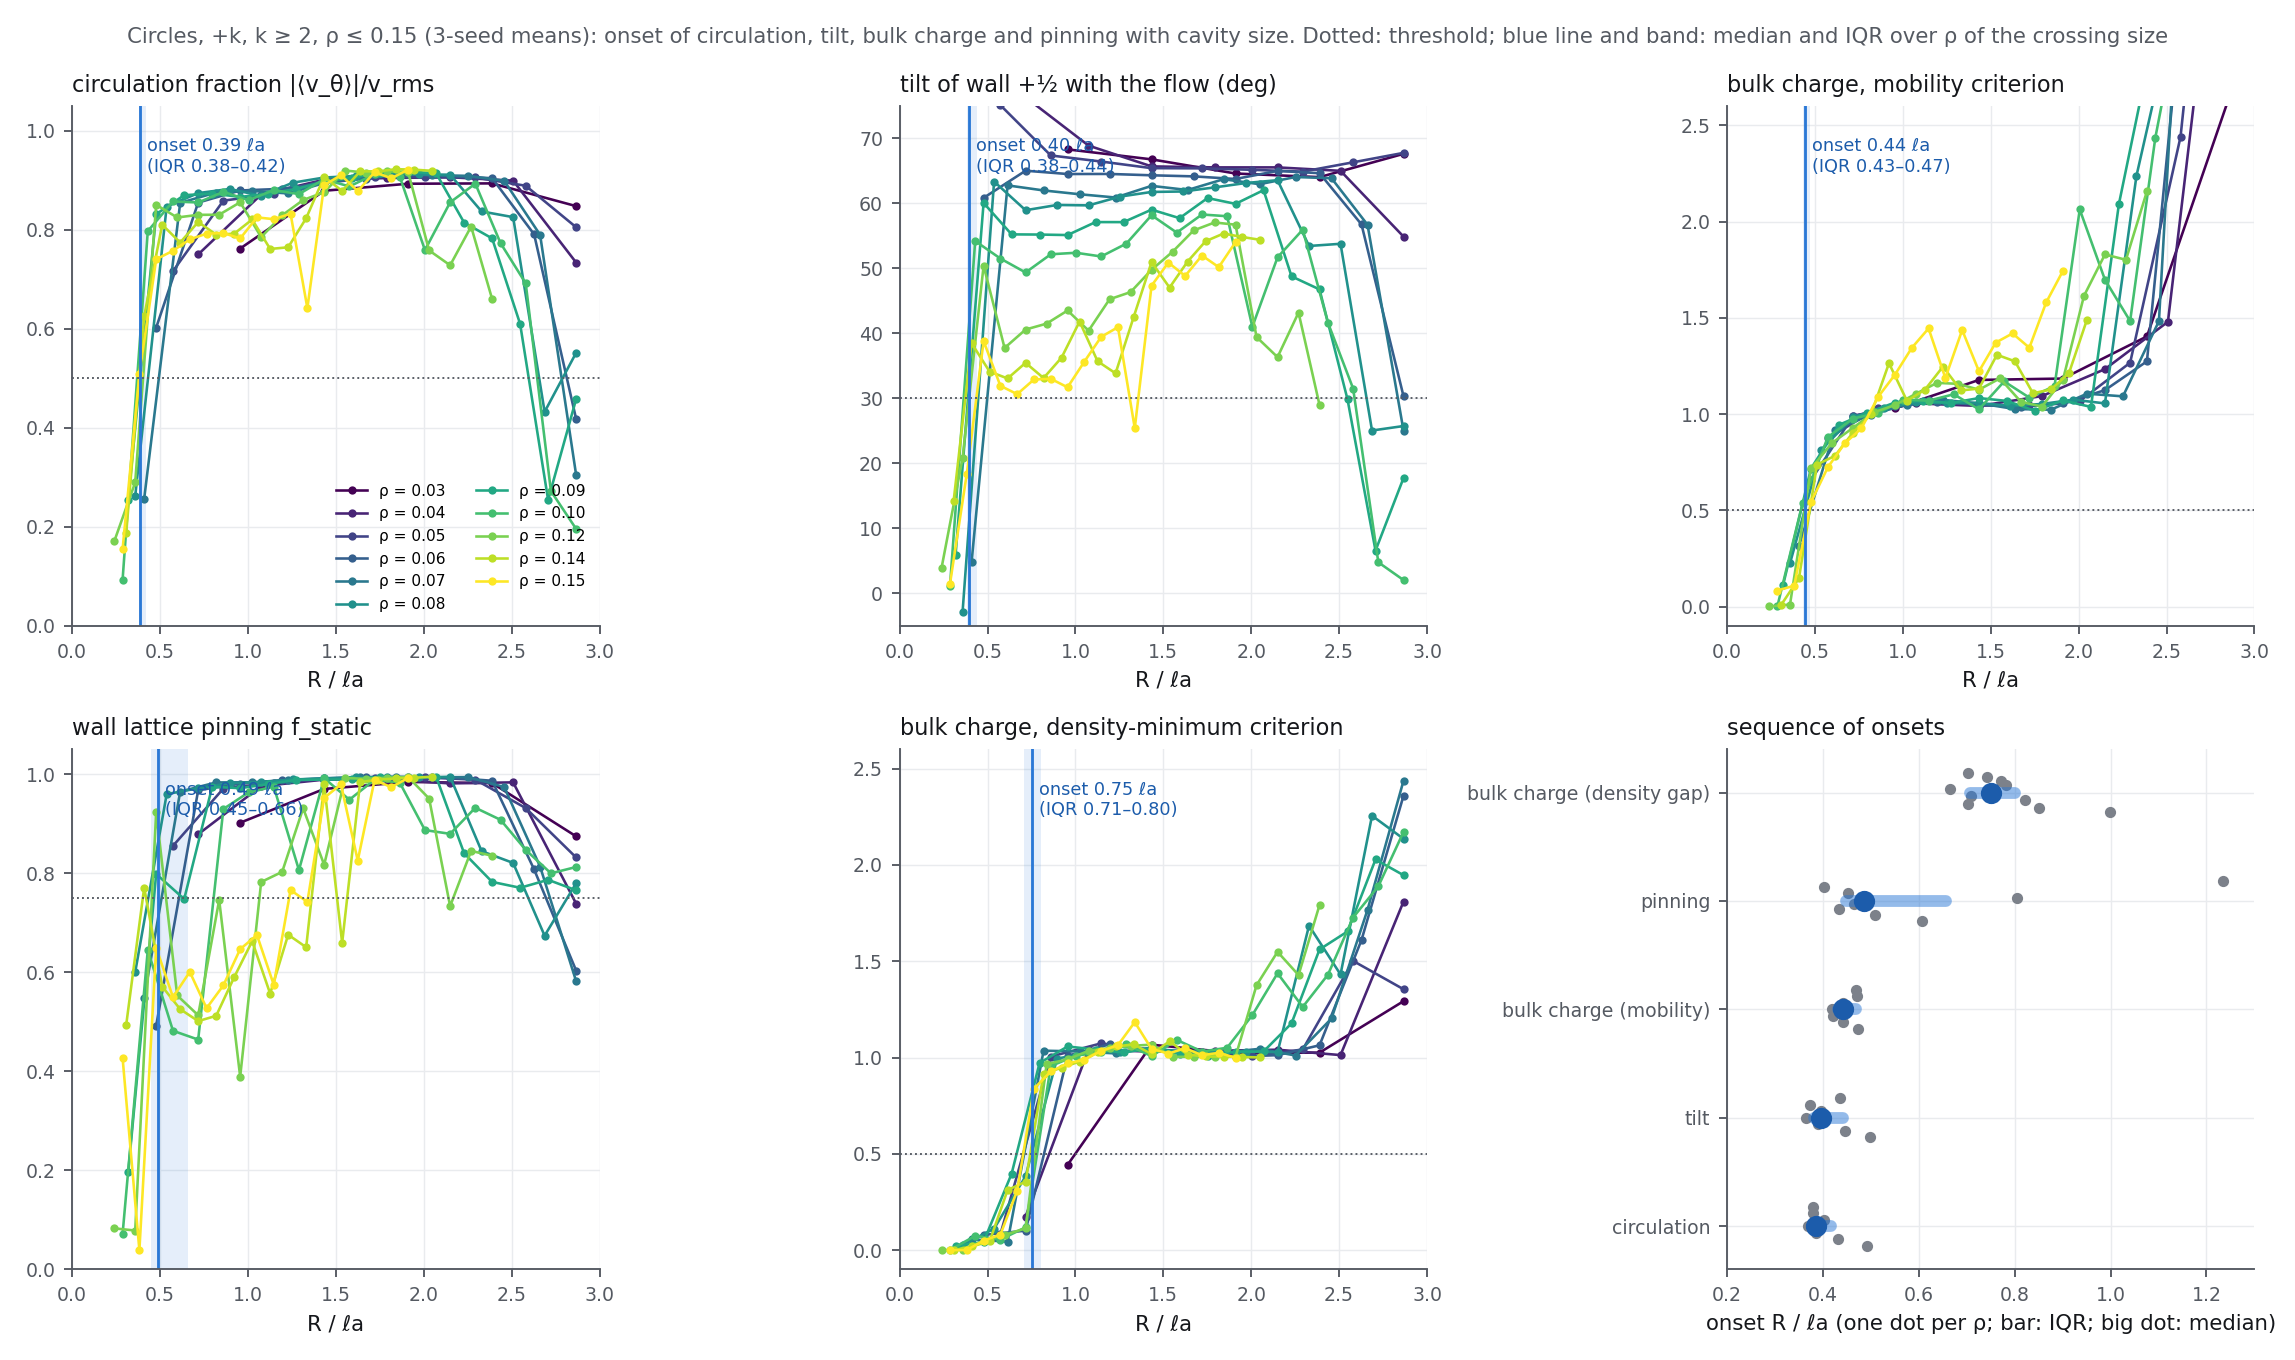
\includegraphics[width=\textwidth]{onset_circles.png}
\caption{\textbf{Onset of the layer/bulk structure in circles} ($+k$, $k\ge2$, $\rho\le0.15$, 3-seed means; one curve per $\rho$).
Circulation fraction $|\langle v_\theta\rangle|/v_\mathrm{rms}$, tilt of the wall $+\half$ signed with the flow, bulk charge from the mobility
criterion, static fraction of the wall lattice, and bulk charge from the density-minimum criterion, against $R/\la$. Dotted: threshold
(0.5, $30^\circ$, 0.5, 0.75, 0.5); blue line and band: median and interquartile range over $\rho$ of the size at which each curve first
crosses it. Last panel: the onsets in order, one dot per $\rho$. Onsets can only be measured for $\rho\ge0.07$, where the sweep has
cavities below $0.5\,\la$ with $k\ge2$.}\label{fig:onset}
\end{figure}
\begin{table}[H]\centering\small
\caption{Onset sizes $R/\la$ per density (\texttt{reports/master/data/onset\_circles.tsv}); ``--'': no crossing within the sweep.}\label{tab:onset}
\begin{tabular}{lccccc}\toprule
$\rho$ & circulation & tilt & bulk charge (mobility) & pinning & bulk charge (density gap)\\\midrule
0.07 & 0.49 & 0.50 & 0.47 & 0.51 & 0.71\\
0.08 & 0.43 & 0.45 & 0.44 & 0.43 & 0.75\\
0.09 & 0.39 & 0.39 & 0.42 & 0.47 & 0.67\\
0.10 & 0.37 & 0.37 & 0.42 & 0.81 & 0.78\\
0.12 & 0.40 & 0.40 & 0.44 & 0.45 & 0.77\\
0.14 & 0.38 & 0.37 & 0.47 & 0.40 & 0.74\\
0.15 & 0.38 & 0.44 & 0.47 & (1.23) & 0.70\\\midrule
median & \textbf{0.39} & \textbf{0.40} & \textbf{0.44} & 0.49 & 0.75\\\bottomrule
\end{tabular}
\end{table}
\begin{itemize}
  \item \textbf{The $+1$ bulk is born with the vortex.} Circulation, the downstream tilt of the wall $+\half$ and the bulk charge
        (mobility) switch on together at $R/\la\approx0.4$ (medians 0.39, 0.40, 0.44), for every density from 0.07 to 0.15. Below that
        size all $2k$ $+\half$ sit at the wall and there is no coherent vortex; above it two $+\half$ leave the wall and the cavity
        circulates. Pinning of the wall lattice follows (median 0.49, scattered), and the density gap between layer and bulk only forms
        at $\approx0.75\,\la$, which is why the density-minimum criterion lags.
  \item \textbf{The upper end mirrors it.} Above $\approx2.3$--$2.5\,\la$ the circulation fraction falls, the tilt vanishes and the bulk charge
        rises above 1 while the wall lattice stays mostly pinned but under-occupied: a \emph{less-charged layer}.
  \item \textbf{Relation to earlier work.} For a wall of charge $+1$, Norton et al.\ found that the onset of circulation occurs at a fixed
        value of $R\sqrt{\alpha}$, i.e.\ at fixed $R/\la$ \cite{TODO_Norton2018}; there the two $+\half$ already exist. Here the wall carries
        all $2k$ imposed $+\half$ below the onset, and the $+1$ bulk is created at the circulation onset, at the same $R/\la$ for every $k$ and
        $\rho$. This supports H4 directly: the bulk charge follows the vortex, at both ends of the size range (and in elongated cavities,
        where the vortex splits, Part~III).
\end{itemize}
\begin{figure}[H]\centering
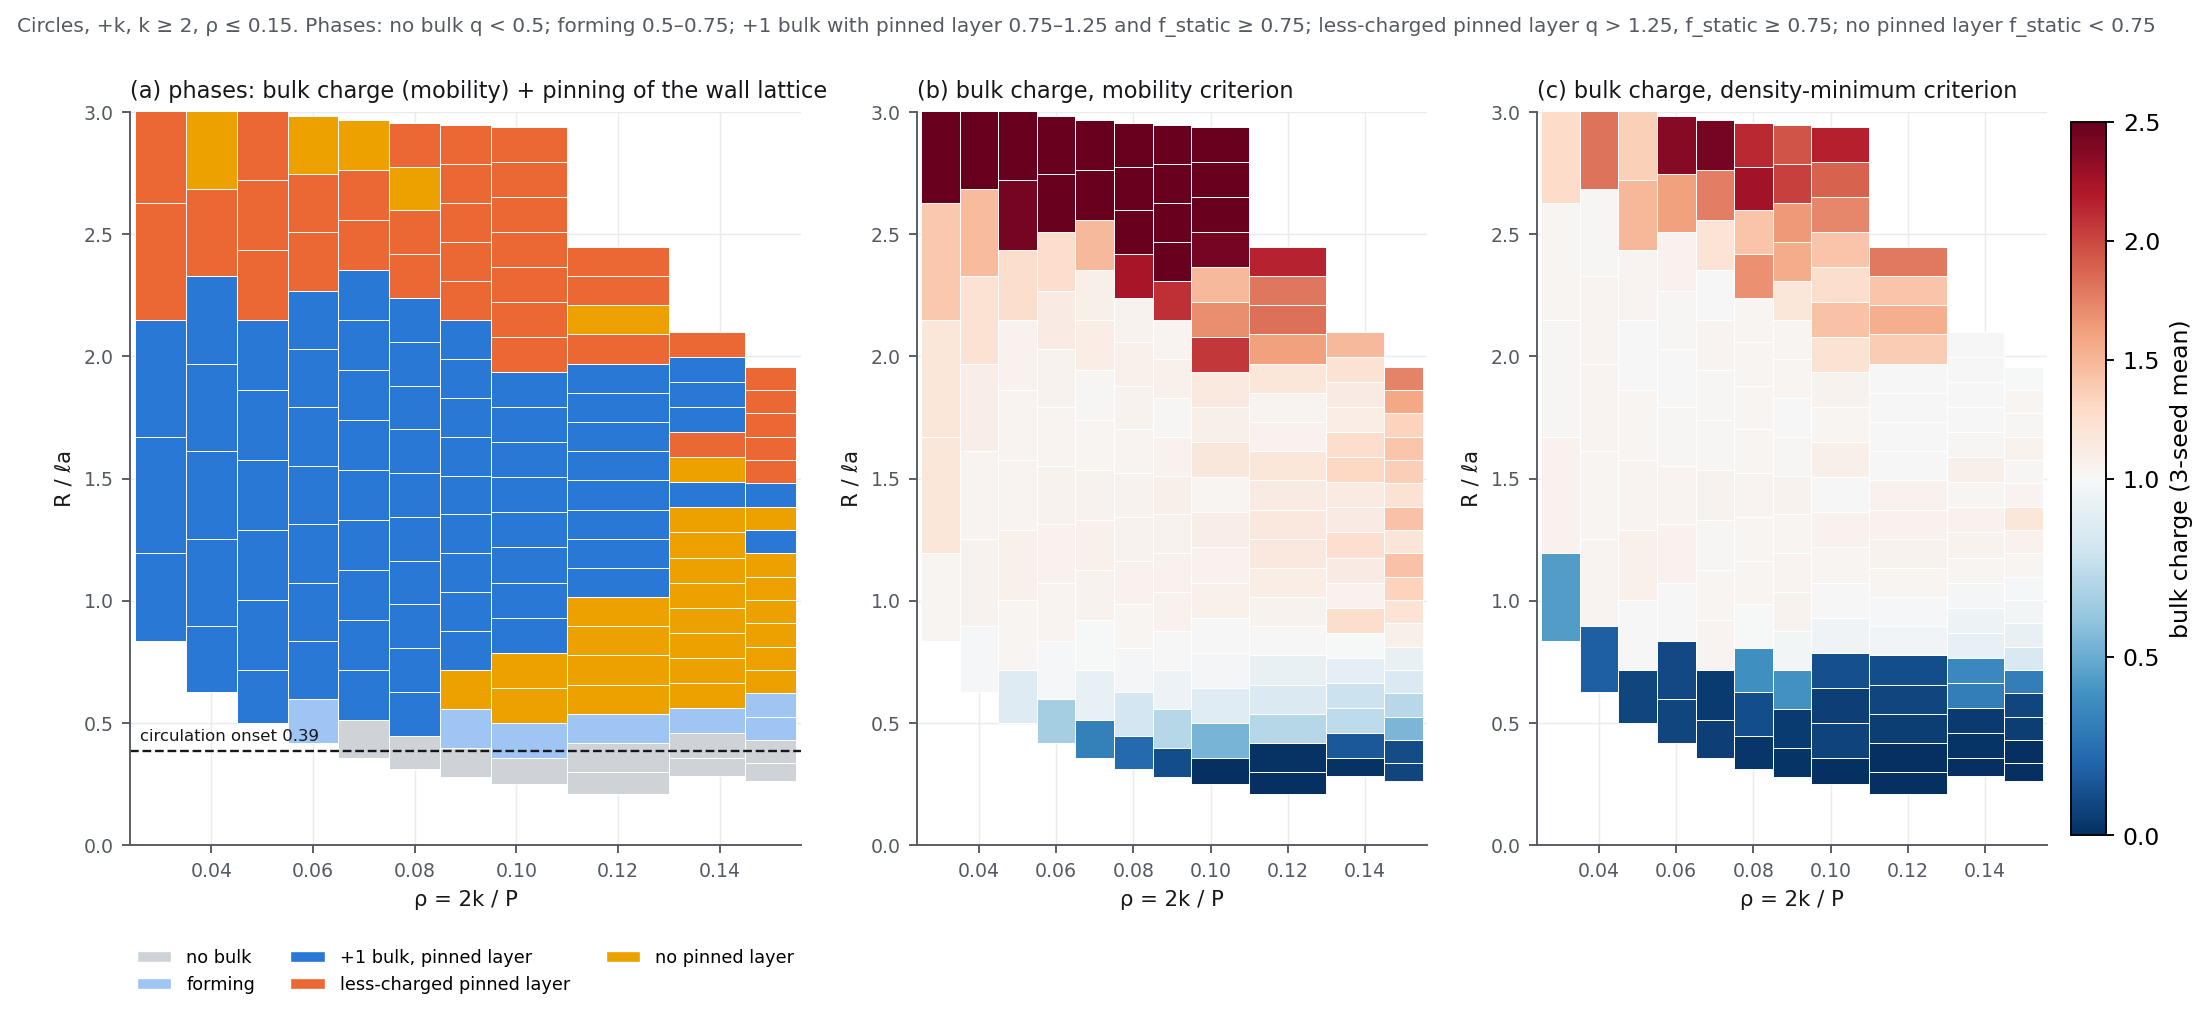
\includegraphics[width=\textwidth]{phase_circles.png}
\caption{\textbf{Phase diagram of circles} ($+k$, $k\ge2$, $\rho\le0.15$, 3-seed means). (a) Phases from the mobility bulk charge $q$
and the static fraction $f_\mathrm{static}$ of the wall lattice: no bulk ($q<0.5$); forming ($0.5\le q<0.75$); $+1$ bulk with a pinned layer
($0.75\le q\le1.25$, $f_\mathrm{static}\ge0.75$); less-charged pinned layer ($q>1.25$, $f_\mathrm{static}\ge0.75$); no pinned layer
($f_\mathrm{static}<0.75$). Dashed: median circulation onset. (b) Bulk charge from the mobility criterion; (c) from the density-minimum
criterion (cross-check), colour centred on 1.}\label{fig:phase}
\end{figure}
\begin{itemize}
  \item 71 of 151 points are $+1$ bulk with a pinned layer, 35 less-charged pinned layer (large $R$), 28 no pinned layer, 17 no bulk or forming.
  \item \textbf{A band without pinning at high density:} for $\rho\ge0.10$ and $R\approx0.5$--$1.4\,\la$ the bulk charge is $\approx1$ but the
        crowded wall lattice keeps rearranging ($f_\mathrm{static}<0.75$; rearrangement times 100--1000, Sec.~\ref{sec:clattice}). Whether this
        is physical or due to the anchoring approaching its resolution limit ($\rho\to0.15$) is open.
  \item The mobility bulk charge sits slightly above 1 (1.05--1.2) inside the $+1$ region, the known bias of this criterion
        (occurrences on broken tracks are skipped; Appendix~\ref{app:issues}); the density-minimum criterion gives 1.00--1.05 there.
\end{itemize}

\subsection{Six bulk-charge criteria over the whole sweep}\label{sec:criteria}
Figures~\ref{fig:critmaps}--\ref{fig:transitions} compare the criteria of Sec.~\ref{sec:edge} on 930 runs ($\rho\le0.15$, both
signs, means over 3 seeds).
\begin{figure}[H]\centering
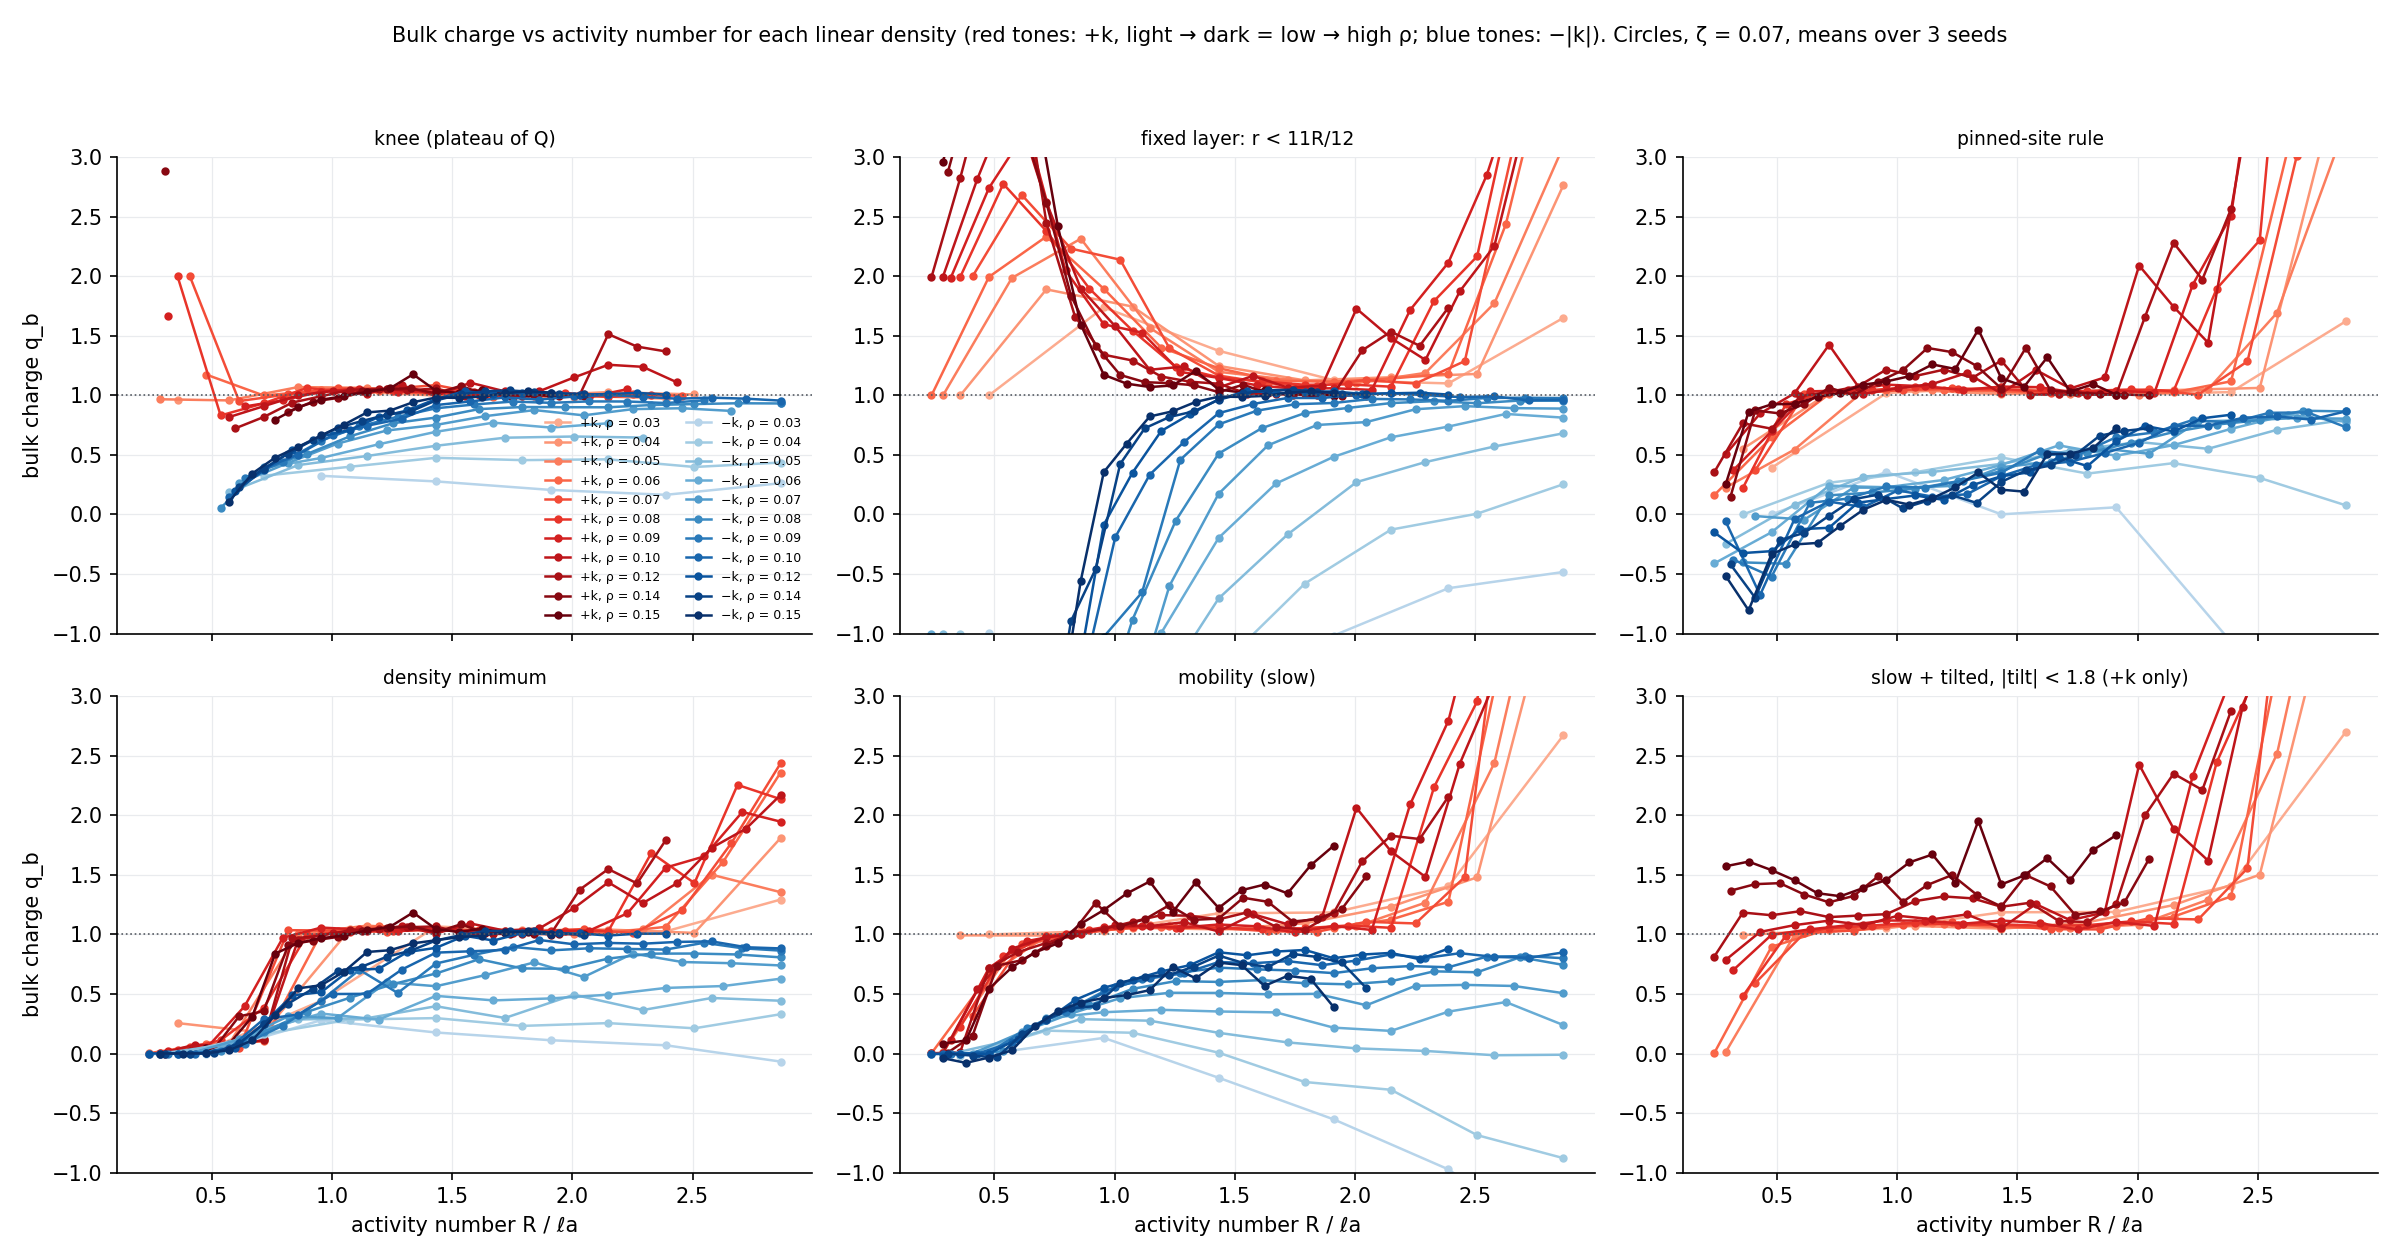
\includegraphics[width=\textwidth]{crit_bulk_vs_R.png}
\caption{Bulk charge against $R/\la$ for six criteria; red tones $+k$ (light to dark: low to high $\rho$), blue tones $-|k|$.}\label{fig:critR}
\end{figure}
\begin{figure}[H]\centering
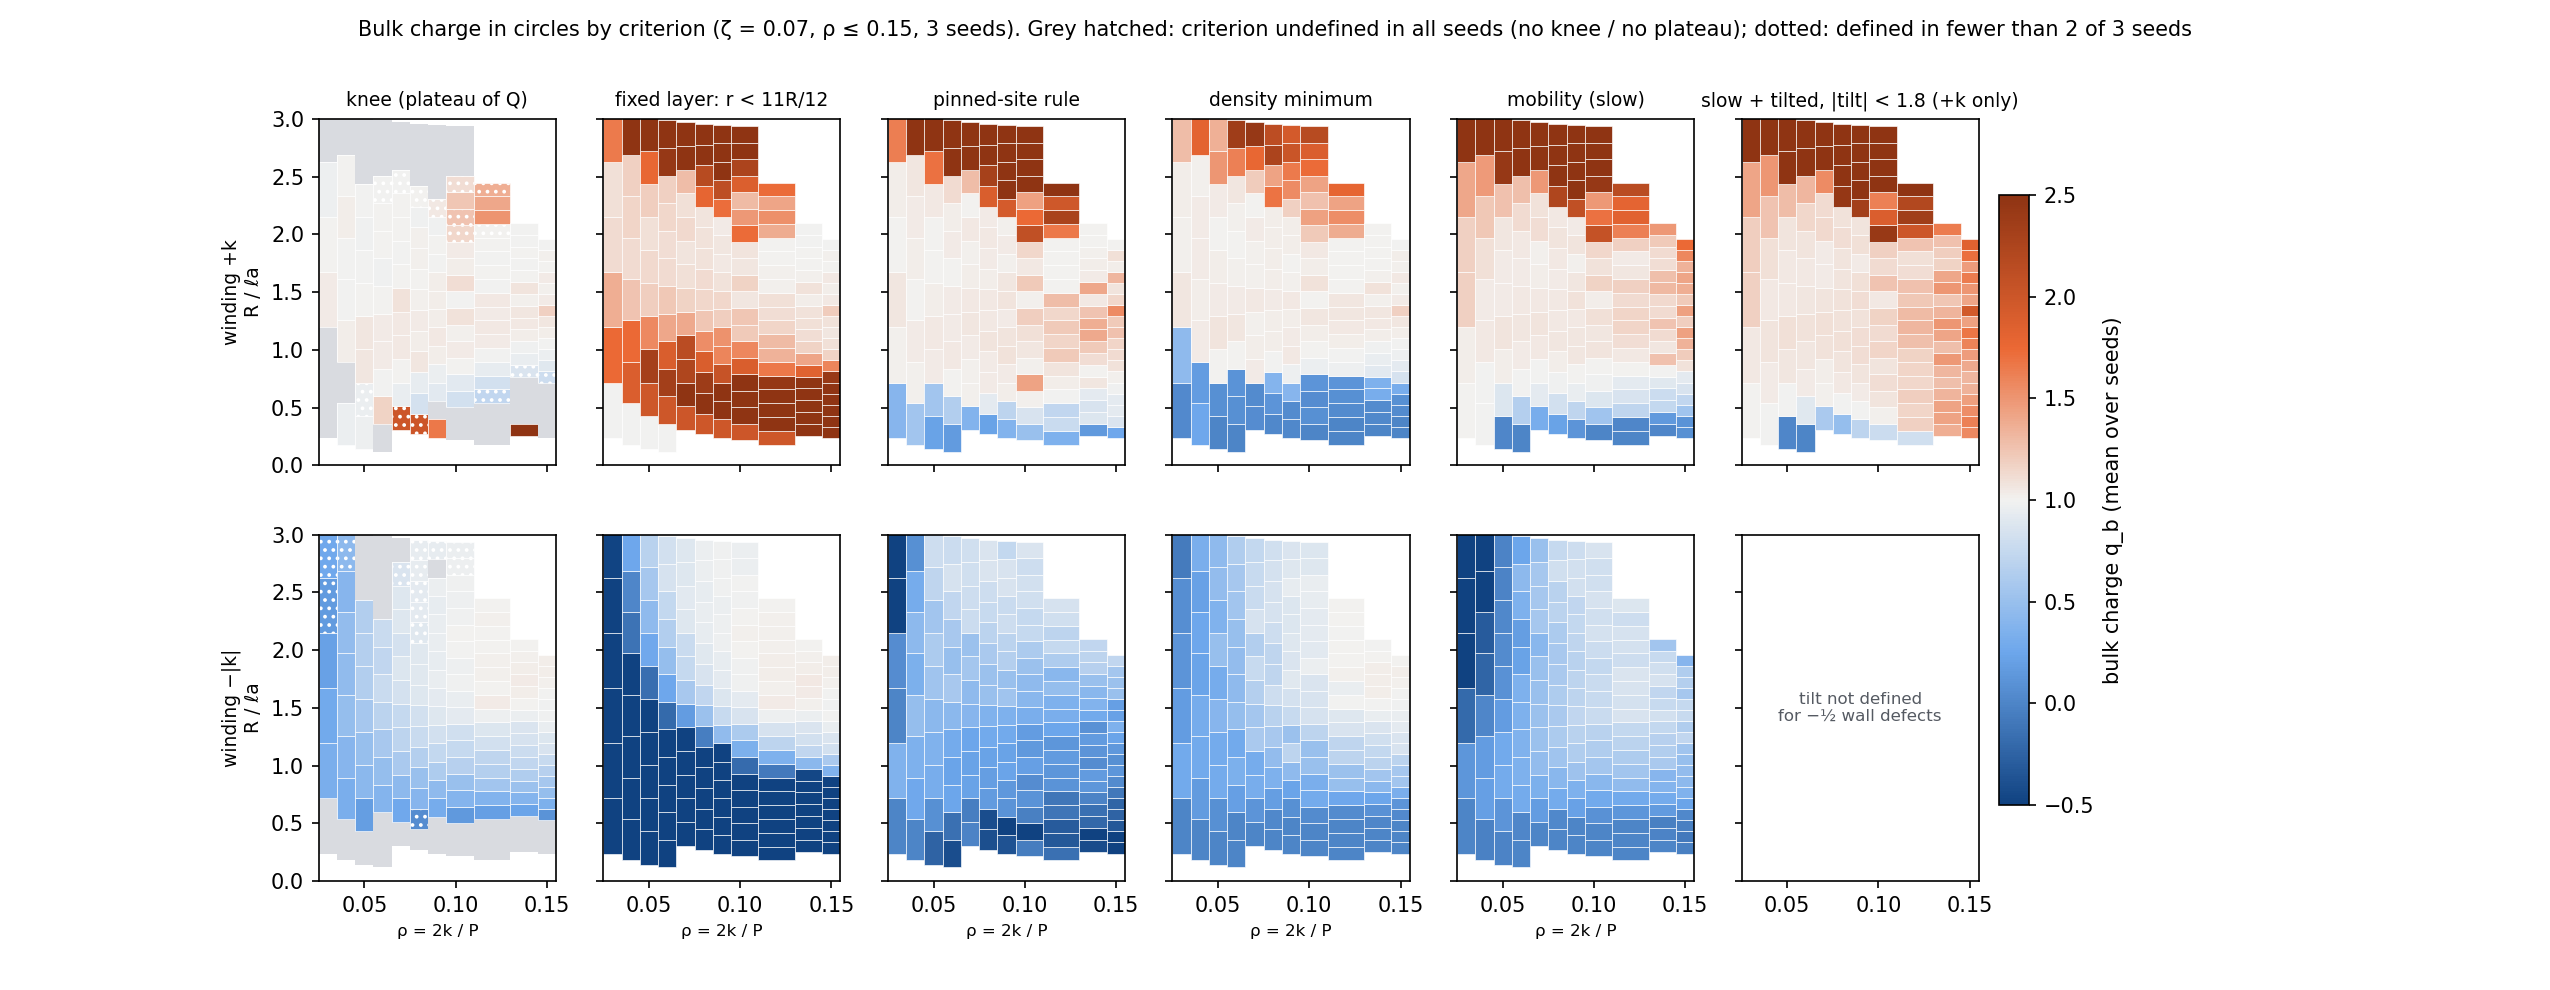
\includegraphics[width=\textwidth]{crit_bulk_maps.png}
\caption{The same as maps over $(\rho,R/\la)$; top $+k$, bottom $-|k|$. Grey hatched: criterion undefined in all seeds (no
knee); dotted: defined in fewer than 2 of 3 seeds.}\label{fig:critmaps}
\end{figure}
\begin{figure}[H]\centering
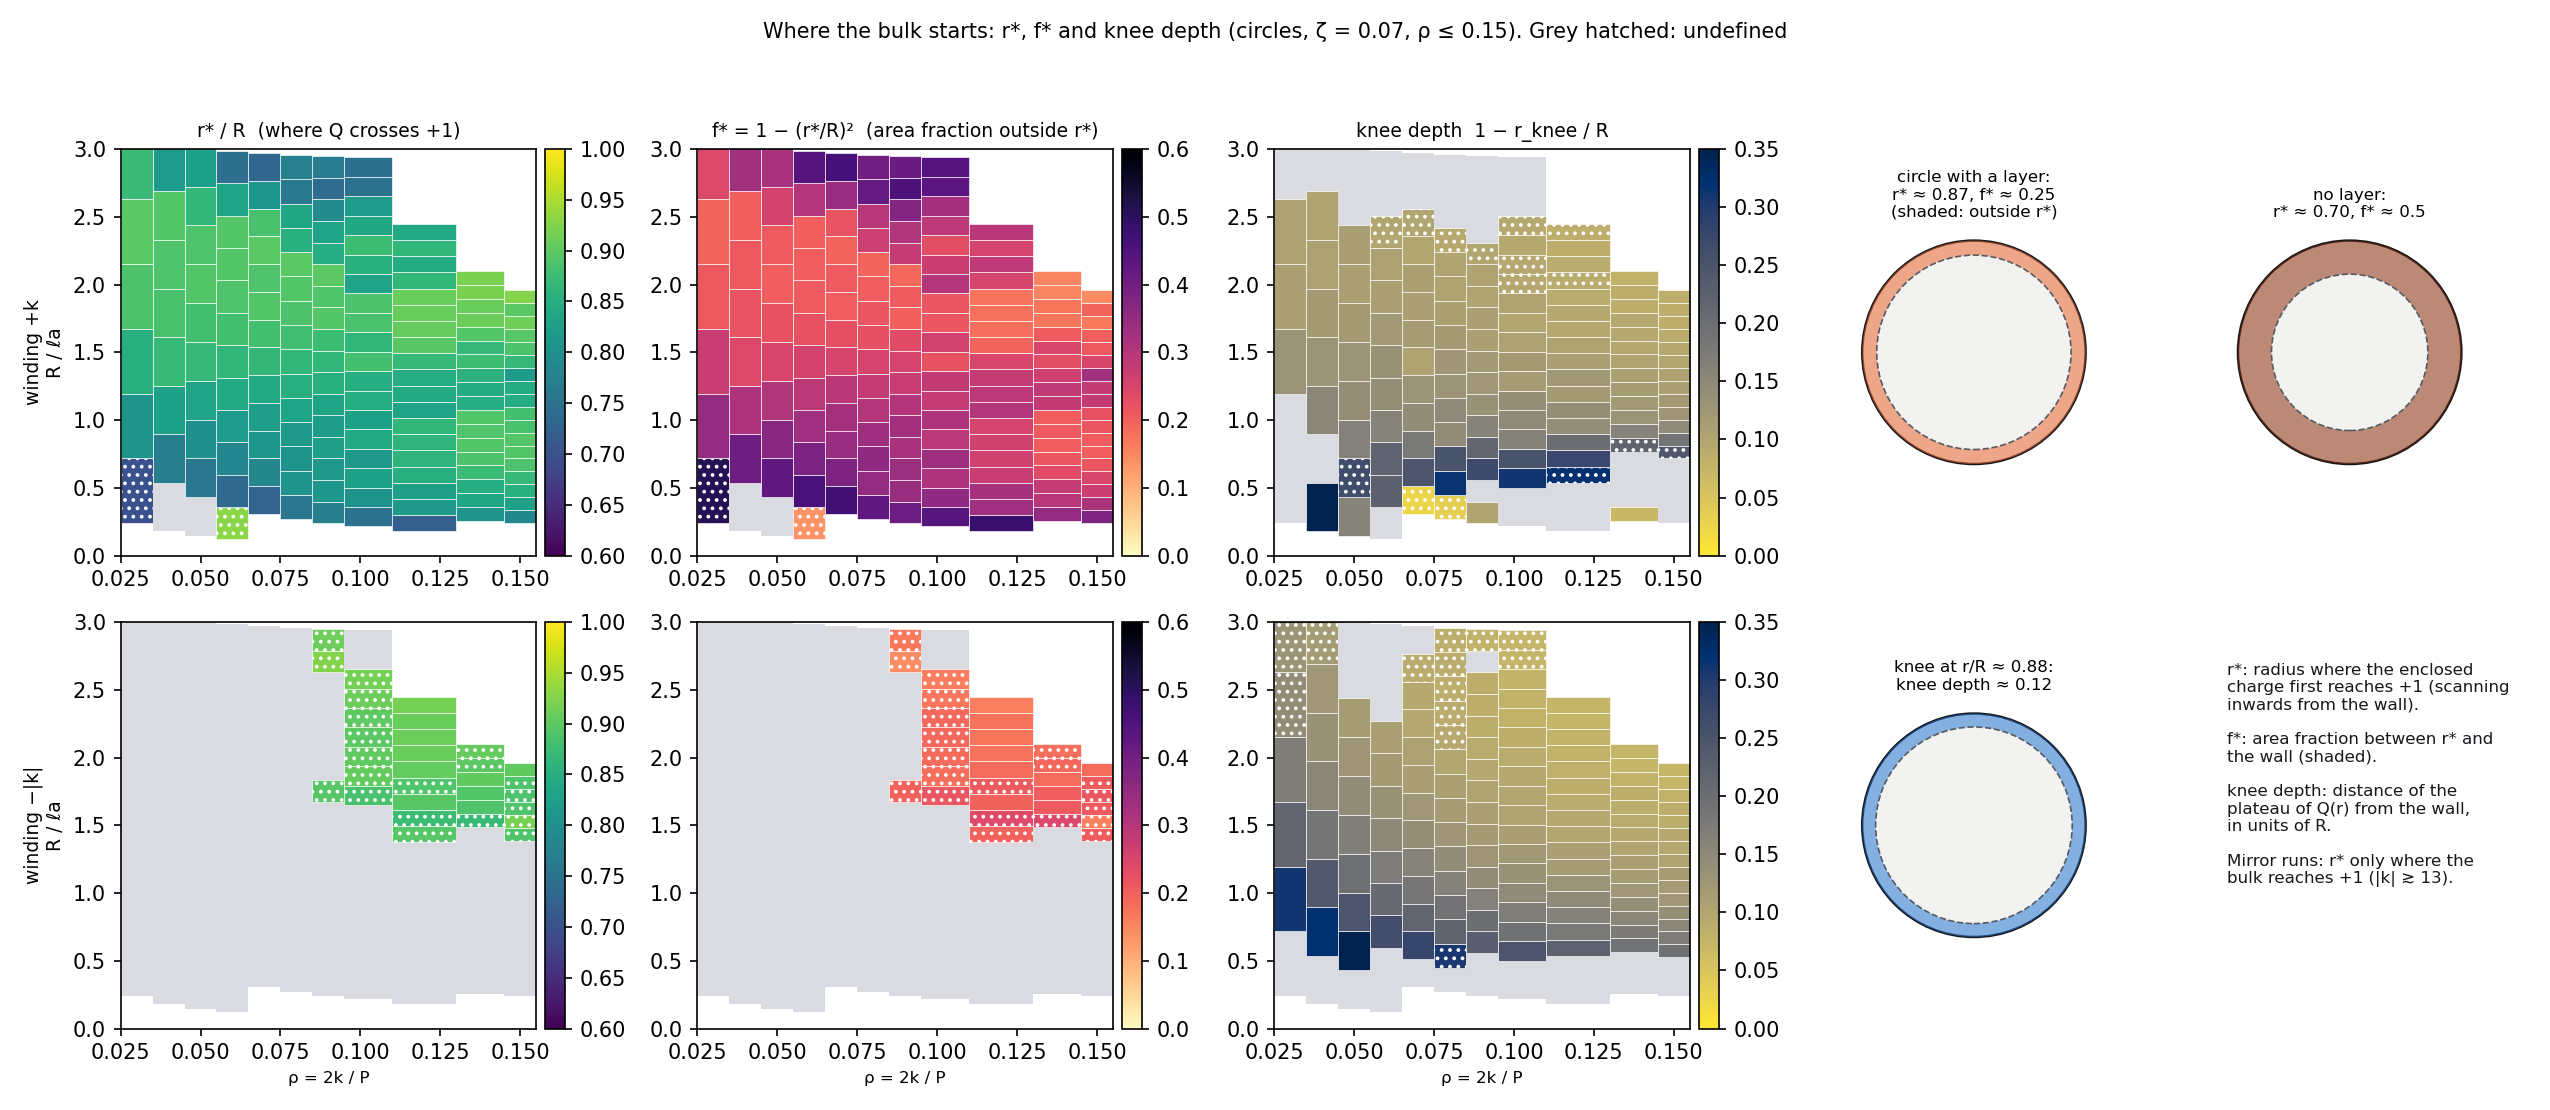
\includegraphics[width=\textwidth]{crit_rstar_fstar_knee.png}
\caption{Where the bulk starts: $r^*/R$ (outermost $Q=+1$ crossing), $f^*=1-(r^*/R)^2$ and the knee depth $1-r_\mathrm{knee}/R$;
top $+k$, bottom $-|k|$ (for $-|k|$, $r^*$ exists only where the bulk reaches $+1$).}\label{fig:rstar}
\end{figure}
\begin{figure}[H]\centering
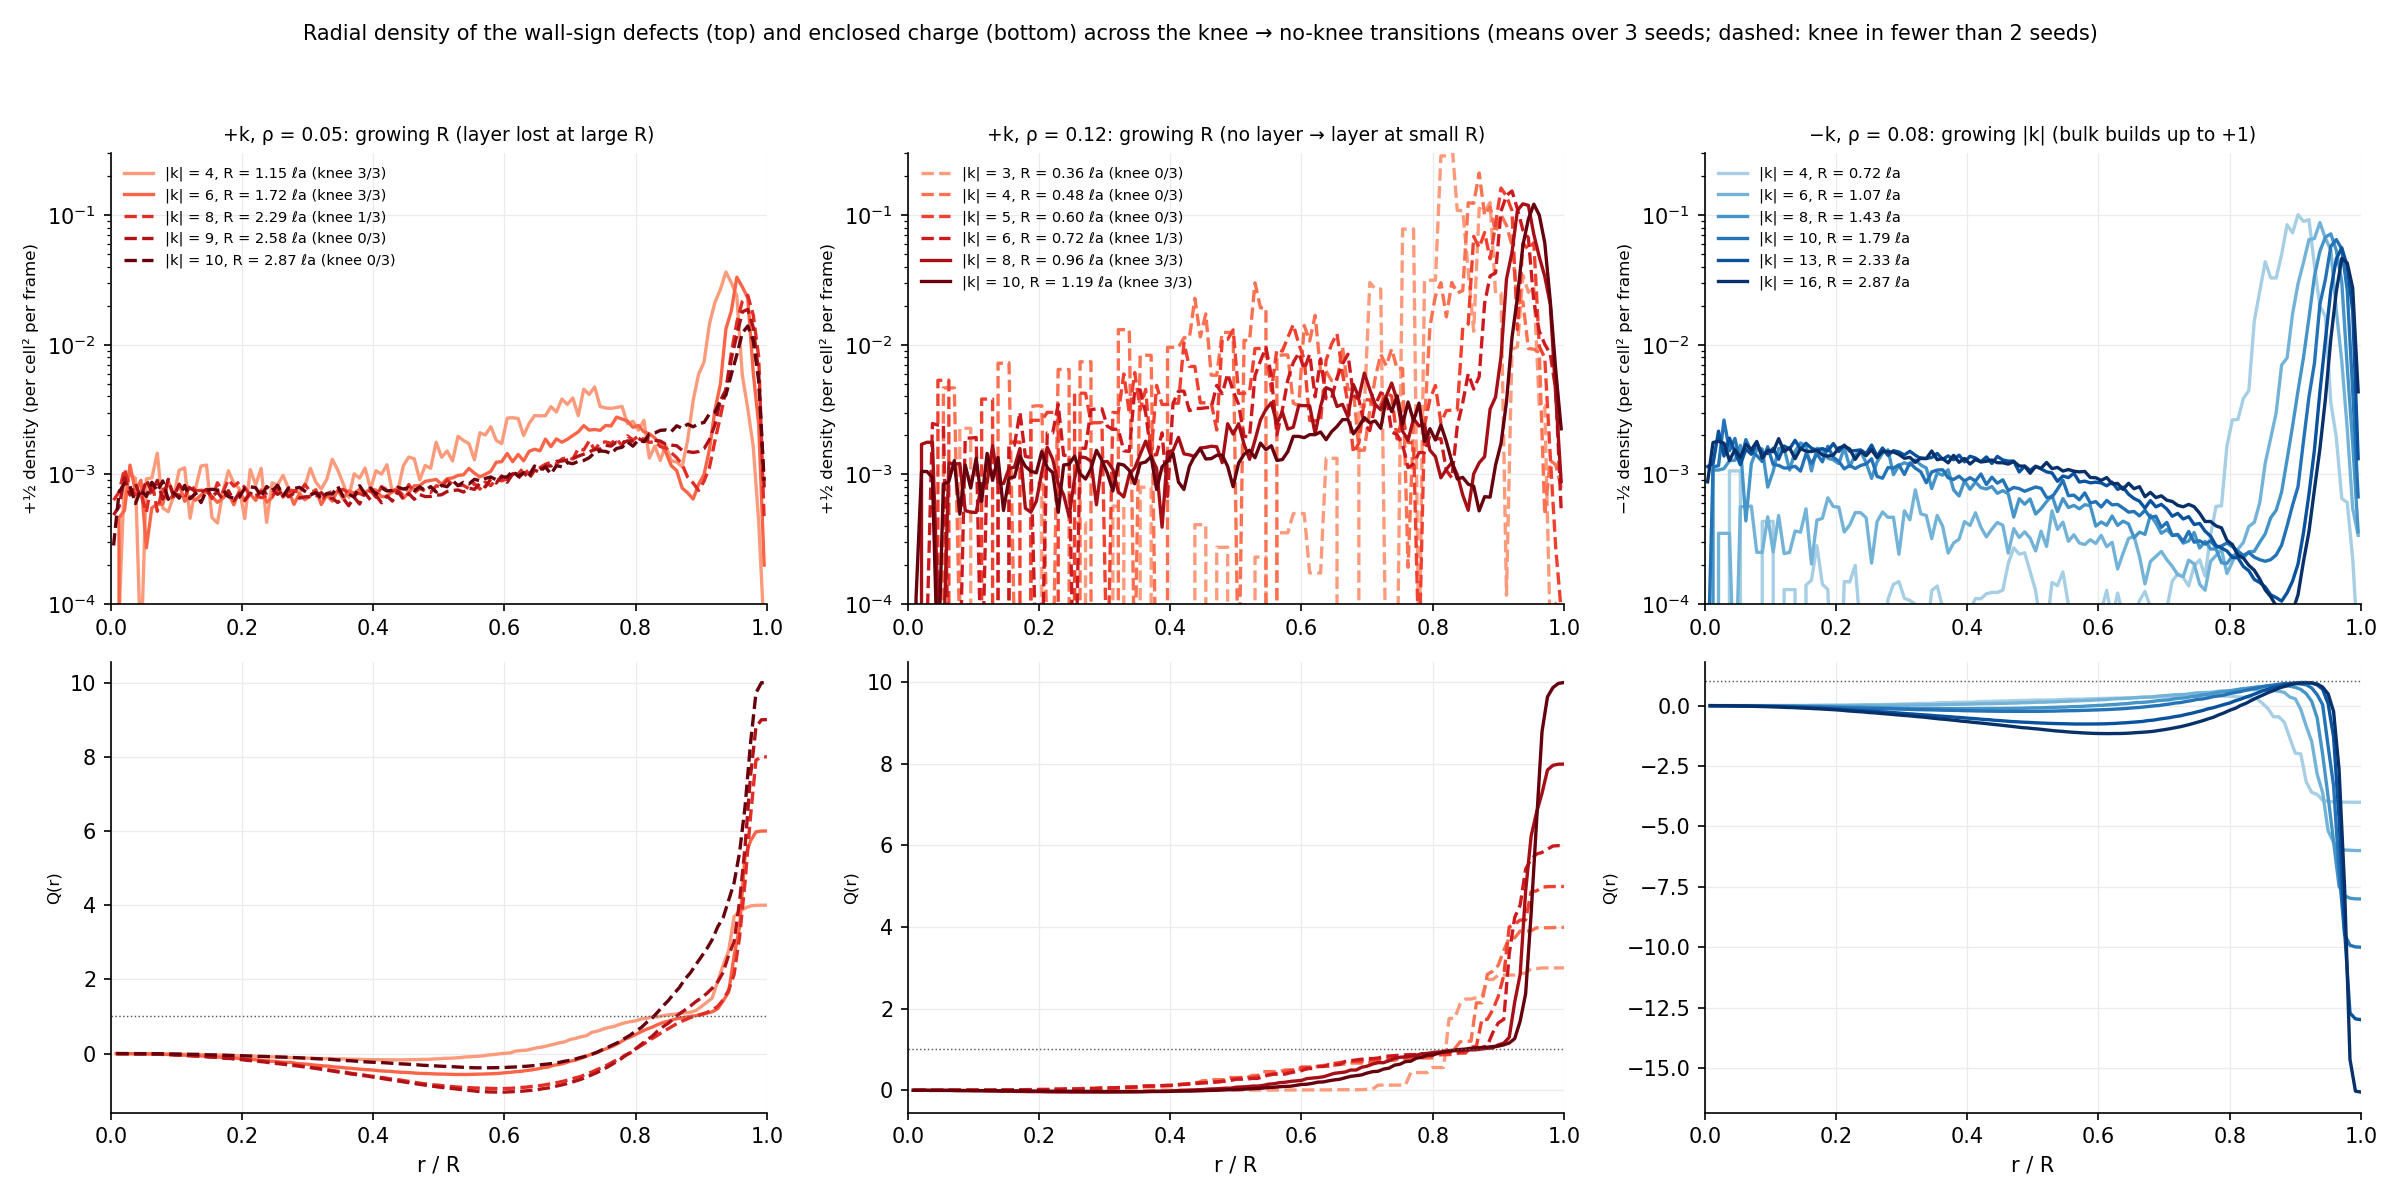
\includegraphics[width=\textwidth]{crit_transitions.png}
\caption{Radial density of the wall-sign defects (top) and $Q(r)$ (bottom) across the knee $\to$ no-knee transitions: $+k$ at
$\rho=0.05$ with growing $R$ (layer lost at large $R$), $+k$ at $\rho=0.12$ (layer appears from $\approx0.96\,\la$), $-k$ at
$\rho=0.08$ with growing $|k|$ (bulk builds up to $+1$). Dashed: knee in fewer than 2 seeds.}\label{fig:transitions}
\end{figure}
\begin{itemize}
  \item \textbf{$+k$:} all criteria agree on $q_b\approx1$ for $R\approx0.8$--$2\,\la$ at every $\rho$. The knee is the most
        robust ($\approx1$ from $\approx0.6$ to $2.4\,\la$) but undefined at large $R$ and low $\rho$. The fixed-depth cut
        ($r<11R/12$) fails at small $R$ (layer thicker than $R/12$: $q_b\gg1$ below $\approx1\,\la$) and at large $R$. Density
        minimum and mobility give $q_b\to0$ below 0.6--0.8\,$\la$ (no bulk defects there). Above 2--2.5\,$\la$ all criteria
        except the knee rise above 1 (defects leave the layer), earliest at high $\rho$. Slow + tilted overcounts (1.3--1.6) at
        high $\rho$, where the wall tilt is smaller (Sec.~\ref{sec:cflow}).
  \item \textbf{$-|k|$:} the knee value rises with $\rho$ and $R$ (0.3--0.5 at $\rho\le0.05$, 0.9--1 only for $\rho\gtrsim0.10$
        and $R\gtrsim1.5\,\la$); site rule and mobility saturate near 0.8 (Sec.~\ref{sec:mirror}).
  \item \textbf{Choice for the paper:} the knee of $Q(r)$ as the primary bulk-charge measure, the density minimum and the
        mobility as cross-checks; no fixed-depth cut.
\end{itemize}
